% Dokumententyp
\documentclass[paper=a4,fontsize=11pt]{scrartcl}

% Packages
\usepackage[T1]{fontenc}
\usepackage[utf8]{inputenc}
\usepackage{setspace}
\usepackage[ngerman]{babel}

\usepackage{amsmath}
\usepackage{amsfonts}
\usepackage{amssymb}
\usepackage{graphicx}
\usepackage[hidelinks]{hyperref}
\usepackage{listings}
\usepackage{float}
\usepackage{rotating}
\usepackage{color}
\usepackage{longtable}
\usepackage{eurosym}
\usepackage{blindtext}

% Deckblatt
% Autor, Titel, Datum
\subject{Hochschule Kempten\\Fakultät Informatik}
\author{}
\titlehead{\centering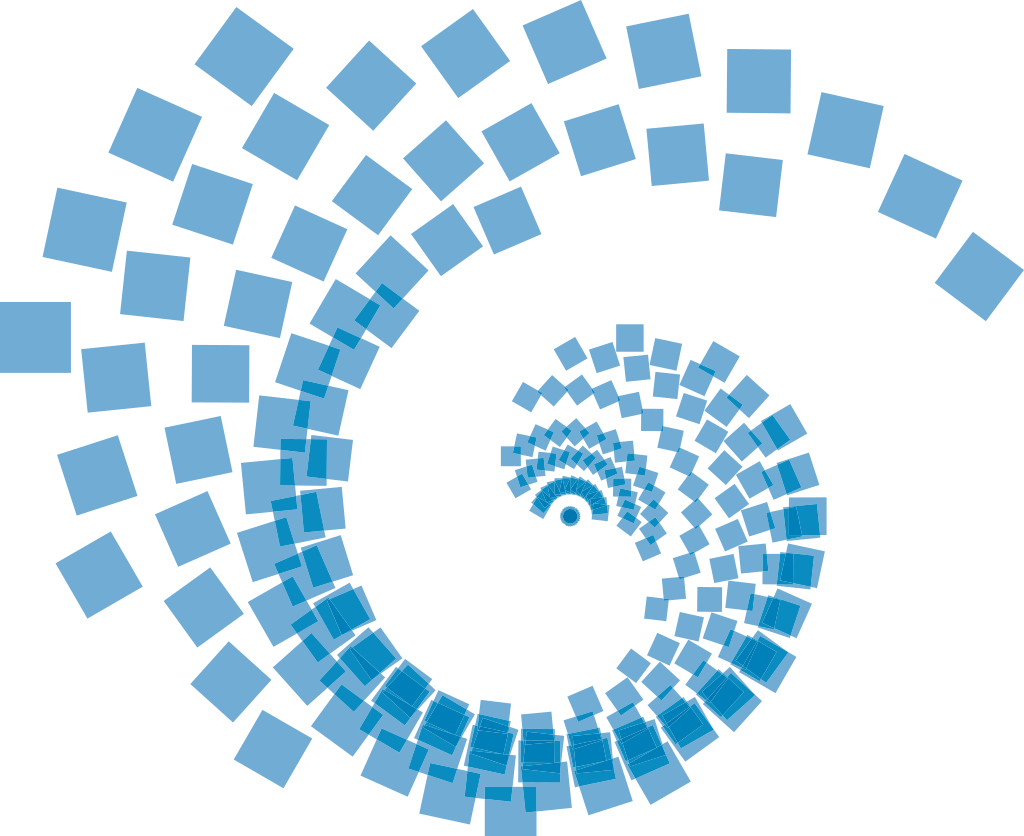
\includegraphics[width=4cm]{img/Logo_HS-Kempten.png}}
\title{Titel des Themas}
\subtitle{Thema: Untertitel}
\date{\today}
\dedication{Autor: Nachname, Vorname\\Matrikel-Nr.: 111111\\Dozent: Prof. Dr. Nachname, Vorname}

%Titel für jede einzelen Seite
%\pagestyle{headings}

% Dokumenten Beginn
\begin{document}
\onehalfspacing

% Deckblatt mit Überschrift ohne Seitenzahl
\maketitle
\thispagestyle{empty}

% Inhaltsverzeichnis
\newpage
\tableofcontents

\newpage

% Inhalt
\section{Kapitel 1}
\subsection{Unterpunkt 1}
\blindtext

\subsection{Unterpunkt 2}
\blindtext

\subsection{Unterpunkt 3}
\blindtext
\cite[Quellenbeschreibung]{001}

\section{Kapitel 2}
\subsection{Unterpunkt 1}
\blindtext
 
\subsection{Unterpunkt 2}
\blindtext

\subsection{Unterpunkt 3}
\blindtext

\newpage

% Quellen- und Literaturverzeichnis
\renewcommand{\refname}{Quellenverzeichnis}
\bibliographystyle{abbrvdin}
\bibliography{Quellenverzeichnis}

% Echtheitserklaerung
\newpage
\thispagestyle{empty}
\section*{Echtheitserklärung}
Ich versichere hiermit, dass die vorliegende Seminararbeit eigenständig und ohne fremde Hilfe verfasst, keine anderen als die angegebenen Quellen verwendet und die den benutzten Quellen entnommenen Passagen als solche kenntlich gemacht wurden. Diese Seminararbeit ist in dieser oder einer ähnlichen Form in keinem anderen Kurs und/oder Studiengang als Studien- oder Prüfungsleistung vorgelegt worden. Hiermit stimmen ich zu, dass die vorliegende Arbeit von der Prüferin/ dem Prüfer in elektronischer Form mit entsprechender Software überprüft wird.

\vspace{25pt} 
\noindent\rule{5cm}{.4pt}\hfill\par 
\noindent Nachname, Vorname

~\\\\
Ort, den {\today}


\end{document}
